\documentclass[11pt]{jarticle}
\usepackage[dvipdfmx]{graphicx}
\usepackage{kcctd-report}
\usepackage{booktabs}
\usepackage{mathcomp}
\usepackage{array}
\usepackage{mathtools,amssymb}
\usepackage{siunitx}
\usepackage{multirow}
\usepackage{tabularx}
\usepackage{subcaption}
\usepackage{float}
\usepackage{listings,jvlisting}
\lstset{
	basicstyle={\ttfamily},
	identifierstyle={\small},
	commentstyle={\smallitshape},
	keywordstyle={\small\bfseries},
	ndkeywordstyle={\small},
	stringstyle={\small\ttfamily},
	frame={tb},
	breaklines=true,
	columns=[l]{fullflexible},
	numbers=left,
	xrightmargin=0zw,
	xleftmargin=3zw,
	numberstyle={\scriptsize},
	stepnumber=1,
	numbersep=1zw,
	lineskip=-0.5ex,
	tabsize=2
}
\renewcommand{\lstlistingname}{ソースコード}

\title{}
\adviser{}

\sdate{令和5年6月29日}
\edate{令和5年7月日}
\fdate{令和5年7月日}
\rdate{西 敬生 教授}

\grade{5}
\anumber{12}
\gnumber{B}
\name{河合 将暉}
\jname{
		岡田 あきたか 川邊 愛貴 きゅうと 久米 りょうと
	  }
\comment{}
\begin{document}
\maketitle

\section{目的}
半導体素子を作成する上で最重要技術である不純物拡散によるシリコンPN接合作成技術を習得し、半導体素子や集積回路の作成技術に関する基本概念を得ることを目的とする.
\section{解説}
	\subsection{拡散}
		異種の粒子が異なった濃度分布で共存するとき,この混合系が熱平衡状態に近づこうとして起こる濃度分布一様化の過程を拡散という.
		拡散を原子の移動という立場から眺めてみると,原子が結晶欠損(穴)に異動するもの,格子間の本来結晶格子がとるべきではない位置へ移動するもの,複数の原子が互いの位置を入れ替えるものがある.
		拡散の過程では,これらが単独に,あるいは組み合わさって起こる.
	\subsection{半導体}
		抵抗率を$10^3~10^9\,\mathrm{\Omega cm}$の範囲に制御できる物質の総称.
		またこの半導体の電気的特性が光,磁気,熱など外部エネルギの影響を強く受ける.
		新聞紙上など,一般的に用いられている場合は,この半導体を材料に作られたICなどのデバイスを指している.
	\subsection{伝導型(p型,n型)}
		半導体中には,マイナスの電荷をもつ電子とプラスの電荷をもつ正孔が存在する.
		2つを合わせて``キャリア''と呼ぶ.
		電子が多い半導体をn型(negativeの頭文字),正孔が多い半導体をp型(positive)と呼ぶ
	\subsection{PN接合}
		p型とn型の半導体が``くっついた''部分に電圧を印加すると整流性が現れる.
	\subsection{ショットキー接触}
		p,nどちらかの半導体と,ある金属を接合させた場合も整流性が現れる.

\section{実験内容}
	\subsection{使用器具}
		\begin{table}[H]
		\begin{center}
		\caption{使用器具}
		\label{tab:used}
		\begin{tabular}{clllll} \toprule
		No&\multicolumn{1}{l}{機器名}&\multicolumn{1}{l}{型番}&\multicolumn{1}{l}{シリアルNo}&\multicolumn{1}{l}{備考}\\ \hline
		1&電気炉&&&\\
		2&ディップコーター&&&\\
		3&真空蒸着装置&&&\\
		4&ホットプレート&&&\\
		5&ジェットオーブン&&&\\
		6&定電圧電源&&&\\
		7&ディジタルマルチメータ&&&\\ \bottomrule
		\end{tabular}
		\end{center}
		\end{table}

	\subsection{実験方法}
		この実験は,拡散現象を利用してシリコン基板中に不純物を混入させ,pn接合を作製した.
		基板の表面からドナーもしくはアクセプタとなる物質を拡散によって混ぜ入れると,表面に近いほど濃度が高い不純物濃度分布となる.
		拡散させた不純物の濃度が基盤自体の不純物濃度に等しくなる深さの位置が,pn接合となる.
		つまり,不純物がアクセプタの場合,不純物混入を行った面がp型,逆側がn型のダイオードの構造となる.

		また,ダイオードを電気回路中に組み込むためには,当然のことながらこれと金属との接触が必要となる.
		しかしながら金属と半導体を単純に接触させると,p型半導体とn型半導体の接触時に作製するショットキー障壁が発生し,この接触部によって新たなダイオードができるので,意図する特性が得られなくなる.
		このため,金属半導体接合部の整流性を排除した抵抗性接触になるようにダイオードに電極を付ける.
		これは,ショットキー障壁の高さを下げるか,壁厚を薄くする(これによりトンネル効果により電流が多く流れるようになる)ことと半導体側のキャリア再結合速度を増大させることで実現できる.
		障壁の厚さは金属の仕事関数の大きさに,壁厚は半導体のキャリア濃度の高さに依存する.
		この実験では,金属の仕事関数を上げる(勢いよく半導体に付着させる)ために,蒸着法を用いた.
		\subsubsection{pn接合試料作成手順}
			\begin{enumerate}
				\item 酸化膜付SiウェーハをFine Crystl Cutterで$1\mathrm{cm} \time 2.5\mathrm{cm}$ぐらいにカット.
				\item ウェーハを洗浄
				\item ディップコータでレジストをウェーハの半分だけ塗布し,保護膜を形成.
				\item ウェーハをバッファードフッ酸の中に入れ,レジストがついていない部分だけ酸化膜エッチング
				\item レジストをアセトン1+第2プロパノール1の混合液とメタノールで除去
				\item P(リン)化合物が解けた不純物溶液を酸化物が除去されたSiウェーハ部分にディップコータで塗布
					  
				\item ホットプレート100~200$^\circ \mathrm{C}$,1分で溶液の乾燥.
				\item 電気炉内で焼成し不純物拡散(1000$^\circ \mathrm{C}$以上 30分)
				\item バッファードフッ酸による不純物ガラス,酸化膜のエッチング
				\item Al蒸着による電極形成
				\item ホットプローブ法によりpn判定で,不純物拡散の出来を確認
				\item 試料の保護のためのスライドガラスをガラス切りによって切断
				\item ロウにより,切断したスライドガラスと試料を接着
			\end{enumerate}
		\subsubsection{測定方法}
			\begin{enumerate}
				\item pn接合ダイオードの順方向・逆方向I−V特性\\
					\begin{enumerate}
						\item 市販のダイオードと電流計,電圧計,直流電圧電流源を接続し,順方向特性について測定した.
							  市販の整流用ダイオードの測定ではしきい電圧の約0.65V以下までは高抵抗素子として,電圧計は電源と並列で,電源は電圧源として測定した.
							  しきい電圧の約0.65V以下までは高抵抗素子として以上は,低抵抗素子として電圧計はダイオードと並列接続し,電源は電流源として測定した.
							  10\,mAになるまで測定した.
						\item 逆方向特性を測定する.20Vぐらいまで電圧を印加したときの電流を確認した.
					\end{enumerate}
				\item 作成したpn接合の順方向・逆方向I−V特性\\
					\begin{enumerate}
						\item 試料表面の電極に測定用針を接触させ,静特性を測定した.
						\item 作成した試料と直流低電圧電流源,電圧計,電流計を接続し順方向のI‐V特性を測定した.
							  このとき,試料の内部抵抗が高いため,以下の全測定において電源は電圧源として使用した.
							  電流が1mAになるまで測定した.(内部抵抗が高いため,しきい電圧以上の電圧を印加する必要がある)
						\item 逆方向特性を測定した.
							  pn接合の降伏現象を確認したいが,内部抵抗が高いため急激な電流の増加は見られないがグラフ化すると傾きが異なるため判明する.
							  そのためグラフがしっかり描けるように測定点を多めに.
					\end{enumerate}
			\end{enumerate}

\section{実験結果}
	\subsection{pn接合ダイオードの順方向・逆方向I−V特性}
		\begin{table}[H]
		\centering
		\caption{既成品pn接合ダイオードの順方向I−V特性(閾値以下)}
		\label{kiseipnunder}
		\begin{minipage}{0.4\columnwidth}
		\centering
		\begin{tabular}{SS} \toprule
			電圧 [mV] & 電流 [$\mathrm{\mu}$A] \\ \hline
			0.000 & 0.06 \\
			49.99 & 0.06 \\
			100.0 & 0.06 \\
			150.0 & 0.08 \\
			200.0 & 0.13 \\
			249.0 & 0.31 \\
			308.8 & 1.11 \\
			318.8 & 1.41 \\
			328.7 & 1.79 \\
			338.7 & 2.31 \\
			348.6 & 3.18 \\
			358.7 & 3.90 \\
			368.6 & 5.07 \\
			378.6 & 6.58 \\
			388.6 & 8.59 \\
			398.5 & 11.80 \\
			408.5 & 14.56 \\
			418.5 & 18.84 \\
			428.4 & 24.25 \\
			438.4 & 31.10 \\
			448.4 & 40.90 \\
			458.3 & 49.82 \\
			468.3 & 62.22 \\
			478.2 & 76.59 \\
			488.2 & 93.59 \\
			498.2 & 116.1 \\
			508.1 & 135.6 \\
			518.1 & 161.2 \\ \bottomrule
			
		\end{tabular}
		\end{minipage}
		\hspace{0.04\columnwidth}
		\begin{minipage}{0.4\columnwidth}
		\centering
		\begin{tabular}{SS} \toprule
			電圧 [mV] & 電流 [$\mathrm{\mu}$A] \\ \hline
			528.1 & 189.6 \\
			538.1 & 220.7 \\
			548.1 & 258.6 \\
			558.0 & 292.3 \\
			568.0 & 332.8 \\
			578.0 & 375.8 \\
			587.9 & 421.8 \\
			597.9 & 474.2 \\
			607.9 & 521.7 \\
			617.8 & 575.8 \\
			629.8 & 642.9 \\
			639.8 & 701.3 \\
			649.8 & 761.0 \\
			659.7 & 823.8 \\
			669.7 & 887.4 \\
			679.6 & 953.1 \\
			689.6 & 1020.2 \\
			699.6 & 1087.4 \\
			709.6 & 1157.6 \\
			719.5 & 1227.2 \\
			729.5 & 1299.5 \\
			739.4 & 1373.0 \\
			749.4 & 1447.1 \\
			759.4 & 1521.0 \\
			769.4 & 1596.2 \\
			779.3 & 1673.1 \\
			789.3 & 1751.4 \\
			799.3 & 1829.2 \\ \bottomrule
		\end{tabular}
		\end{minipage}
		\end{table}

		\begin{table}[H]
		\begin{center}
		\caption{既成品pn接合ダイオードの順方向I−V特性(閾値以上)}
		\label{tab:kiseipnover}
		\begin{tabular}{SS} \toprule
			電流 [mA] & 電圧 [V] \\ \hline
			0.9996 & 0.5838 \\
			1.099 & 0.5883 \\
			1.199 & 0.5921 \\
			1.300 & 0.5958 \\
			1.400 & 0.5990 \\
			1.499 & 0.6022 \\
			1.599 & 0.6051 \\
			1.699 & 0.6077 \\
			1.799 & 0.6099 \\
			1.899 & 0.6122 \\
			1.999 & 0.6130 \\
			9.996 & 0.6900 \\
			19.989 & 0.7201 \\
			29.988 & 0.7371 \\
			39.984 & 0.7489 \\
			49.984 & 0.7579 \\
			59.96 & 0.7652 \\
			69.95 & 0.7712 \\
			79.94 & 0.7763 \\
			89.93 & 0.7806 \\
			99.93 & 0.7846 \\ \bottomrule
		\end{tabular}
		\end{center}
		\end{table}

		\begin{table}[H]
		\begin{center}
		\caption{既成品pn接合ダイオードの逆方向I−V特性}
		\label{kiseipngyaku}
		\begin{tabular}{SS} \toprule
			電圧 [mV] & 電流 [$\mathrm{\mu}$A] \\ \hline
			-0.640 & 0.06 \\
			-49.36 & 0.06 \\
			-99.30 & 0.06 \\
			-144.18 & 0.06 \\
			-199.06 & 0.06 \\
			-248.91 & 0.06 \\
			-298.78 & 0.06 \\
			-348.56 & 0.06 \\
			-448.31 & 0.06 \\
			-498.15 & 0.06 \\
			-548.1 & 0.06 \\
			-597.9 & 0.06 \\
			-649.8 & 0.06 \\
			-5000 & 0.06 \\
			-10000 & 0.06 \\
			-20000 & 0.06 \\
			-25000 & 0.06 \\ \bottomrule
		\end{tabular}
		\end{center}
		\end{table}

	\subsection{作成したpn接合の順方向・逆方向I−V特性}

	\begin{table}[H]
	\begin{center}
	\caption{引き上げ速度1\,mm/sにおけるpn接合の順方向I−V特性1}
	\label{tab:jisakupnjun1}
	\begin{tabular}{SS} \toprule
		電圧[V] & 電流[μA] \\ \hline
		0.0000 & -71.95 \\
		0.1991 & -34.33 \\
		0.2191 & -14.50 \\
		0.2490 & -5.970 \\
		0.2988 & 23.95 \\
		0.3496 & 59.33 \\
		0.3995 & 88.90 \\
		0.4194 & 101.8 \\
		0.4394 & 115.8 \\
		0.4593 & 129.6 \\
		0.4793 & 143.6 \\
		0.4992 & 159.6 \\
		0.5191 & 176.2 \\
		0.5391 & 192.2 \\
		0.5590 & 209.6 \\
		0.5789 & 228.1 \\
		0.5989 & 246.7 \\
		0.7993 & 485.4 \\
		0.9996 & 808.2 \\ \bottomrule
	\end{tabular}
	\end{center}
	\end{table}

	\begin{table}[H]
	\begin{center}
	\caption{引き上げ速度1\,mm/sにおけるpn接合の逆方向I−V特性1}
	\label{tab:jisakupngyaku1}
	\begin{tabular}{SS} \toprule
		電圧[V] & 電流[mA] \\ \hline
		-0.0002 & -0.056 \\
		-0.9997 & -0.089 \\
		-2.000 & -0.103 \\
		-2.999 & -0.114 \\
		-3.999 & -0.142 \\
		-4.999 & -0.194 \\
		-5.199 & -0.220 \\
		-5.400 & -0.307 \\
		-5.599 & -0.407 \\
		-5.799 & -0.513 \\
		-6.001 & -0.623 \\
		-6.199 & -0.728 \\
		-6.400 & -0.841 \\
		-6.599 & -0.953 \\
		-6.800 & -1.072 \\
		-7.000 & -1.187 \\
		-8.000 & -1.845 \\
		-9.000 & -2.518 \\
		-10.00 & -3.208 \\ \bottomrule
	\end{tabular}
	\end{center}
	\end{table}

	\begin{table}[H]
	\begin{center}
	\caption{引き上げ速度1\,mm/sにおけるpn接合の順方向I−V特性2}
	\label{tab:jisakupnjun2}
	\begin{tabular}{SS} \toprule
		電圧[V] & 電流[mA] \\ \hline
		0.0000 & -52.45 \\
		0.1991 & -21.37 \\
		0.2499 & -0.820 \\
		0.2988 & 50.16 \\
		0.3496 & 138.6 \\
		0.3995 & 249.1 \\
		0.4493 & 379.3 \\
		0.4992 & 530.3 \\
		0.5490 & 695.8 \\
		0.5989 & 872.7 \\
		0.7993 & 1666.6 \\
		0.9997 & 2533.6 \\ \bottomrule
	\end{tabular}
	\end{center}
	\end{table}

	\begin{table}[H]
	\begin{center}
	\caption{引き上げ速度1\,mm/sにおけるpn接合の逆方向I−V特性2}
	\label{tab:jisakupngyaku2}
	\begin{tabular}{SS} \toprule
		電圧[V] & 電流[mA] \\ \hline
		0.000 & -0.048 \\
		-1.000 & -0.062 \\
		-1.999 & -0.073 \\
		-2.999 & -0.111 \\
		-3.999 & -0.16 \\
		-4.499 & -0.226 \\
		-4.999 & -0.267 \\
		-5.500 & -0.337 \\
		-6.000 & -0.415 \\
		-7.000 & -0.588 \\
		-8.000 & -0.793 \\
		-9.000 & -1.016 \\
		-10.00 & -1.263 \\ \bottomrule
	\end{tabular}
	\end{center}
	\end{table}

	\begin{table}[H]
	\begin{center}
	\caption{引き上げ速度0.1\,mm/sにおけるpn接合の順方向I−V特性}
	\label{tab:jisakupnjun0.1}
	\begin{tabular}{SS} \toprule
		電圧[V] & 電流[μA] \\ \hline
		0.002 & -40.89 \\
		0.1991 & -2.120 \\
		0.2090 & 0.07 \\
		0.2191 & 6.950 \\
		0.2290 & 17.13 \\
		0.2390 & 24.75 \\
		0.2490 & 35.18 \\
		0.2589 & 41.82 \\
		0.2689 & 53.44 \\
		0.2789 & 65.74 \\
		0.2888 & 78.69 \\
		0.3197 & 123.1 \\
		0.3397 & 158.1 \\
		0.3596 & 193.7 \\
		0.3796 & 231.1 \\
		0.3995 & 272.7 \\
		0.5989 & 768.8 \\
		0.7993 & 1373.1 \\
		0.9997 & 2033.4 \\ \bottomrule
	\end{tabular}
	\end{center}
	\end{table}

	\begin{table}[H]
	\begin{center}
	\caption{引き上げ速度0.1\,mm/sにおけるpn接合の逆方向I−V特性}
	\label{tab:jisakupngyaku0.1}
	\begin{tabular}{SS} \toprule
		電圧[V] & 電流[mA] \\ \hline
		0.000 & -0.0490 \\
		-1.000 & -0.0750 \\
		-2.000 & -0.1200 \\
		-3.000 & -0.1760 \\
		-4.000 & -0.2660 \\
		-5.000 & -0.3770 \\
		-5.499 & -0.4430 \\
		-6.001 & -0.5200 \\
		-6.500 & -0.5910 \\
		-7.000 & -0.6810 \\
		-8.000 & -0.8750 \\
		-9.000 & -1.265 \\
		-10.00 & -1.835 \\ \bottomrule
	\end{tabular}
	\end{center}
	\end{table}

	\begin{figure}[H]
	\centering
	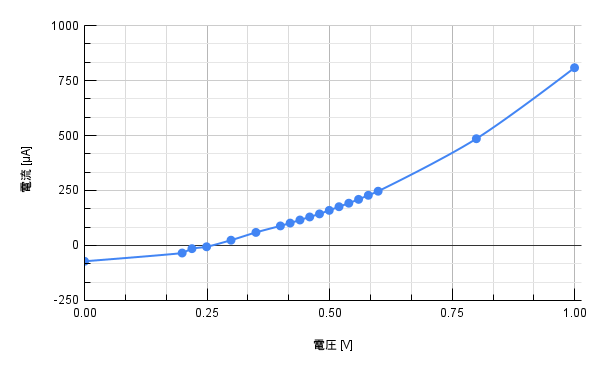
\includegraphics[width = 12cm]{figs/chart1.png}
	\caption{引き上げ速度1\,mm/sにおけるpn接合の順方向I−V特性図1}
	\label{fig:pnjun1}
	\end{figure}

	\begin{figure}[H]
	\centering
	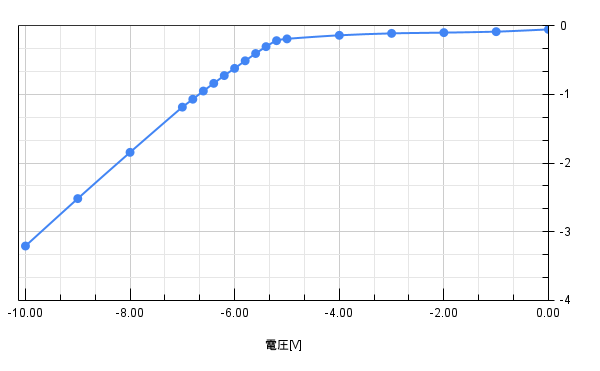
\includegraphics[width = 12cm]{figs/chart4.png}
	\caption{引き上げ速度1\,mm/sにおけるpn接合の逆方向I−V特性図1}
	\label{fig:pngyaku1}
	\end{figure}

	\begin{figure}[H]
	\centering
	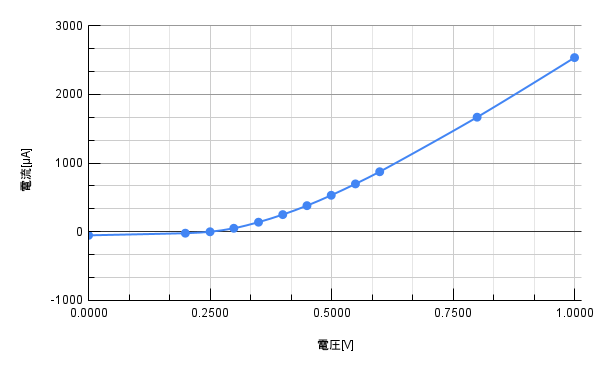
\includegraphics[width = 12cm]{figs/chart2.png}
	\caption{引き上げ速度1\,mm/sにおけるpn接合の順方向I−V特性図2}
	\label{fig:pnjun2}
	\end{figure}

	\begin{figure}[H]
	\centering
	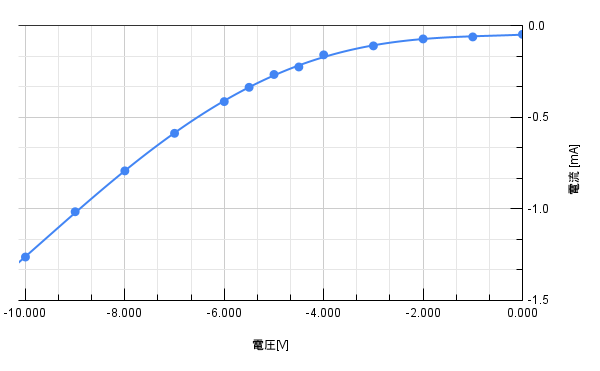
\includegraphics[width = 12cm]{figs/chart5.png}
	\caption{引き上げ速度1\,mm/sにおけるpn接合の逆方向I−V特性図2}
	\label{fig:pngyaku2}
	\end{figure}

	\begin{figure}[H]
	\centering
	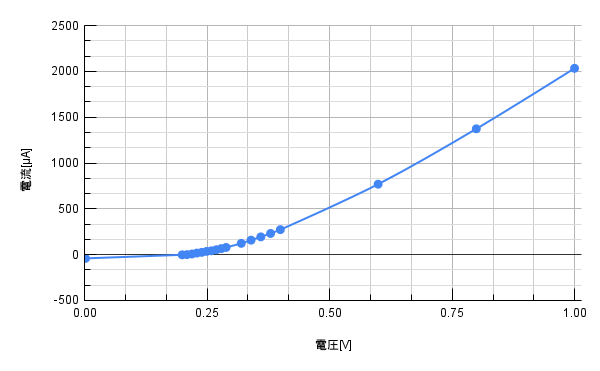
\includegraphics[width = 12cm]{figs/chart3.png}
	\caption{引き上げ速度0.1\,mm/sにおけるpn接合の順方向I−V特性図}
	\label{fig:pnjun0.1}
	\end{figure}

	\begin{figure}[H]
	\centering
	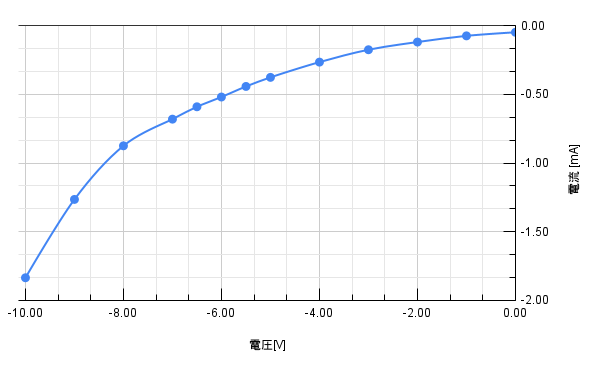
\includegraphics[width = 12cm]{figs/chart6.png}
	\caption{引き上げ速度0.1\,mm/sにおけるpn接合の逆方向I−V特性図}
	\label{fig:pngyaku0.1}
	\end{figure}

\section{考察}
	\subsection{pn判定}
	\subsection{I−V特性}
	\subsection{片対数の結果}
\section{感想}

\begin{thebibliography}{99}
\bibitem{ref:指導書}
西 敬生「実験実習指導書」神戸高専電子工学科 pp.15-16
\end{thebibliography}
\end{document}